\documentclass{article}

\newcommand{\ep}{\rule{.06in}{.1in}}
\textheight 9.5in

\usepackage{amssymb, bm}
\usepackage{amsmath}
\usepackage{amsthm}
\usepackage{graphicx, subcaption, booktabs}

\usepackage{tikz, pgfplots, pgfplotstable, chemfig, xcolor}

% \usepgfplotslibrary{colorbrewer, statistics}
% \pgfplotsset{
%   exact axis/.style={grid=major, minor tick num=4, xlabel=$v^*$,
%     legend entries={PDF, CDF},},
%   every axis plot post/.append style={thick},
%   table/search
%   path={/Users/andrewwork/thesis/jump-velocity/dat-files},
%   colormap/YlGnBu,
%   cycle list/Set1-5,
%   legend style={legend cell align=left,},
% }

% \usepgfplotslibrary{external}
% \tikzexternalize

\renewcommand{\arraystretch}{1.2}
\pagestyle{empty} 
\oddsidemargin -0.25in
\evensidemargin -0.25in 
\topmargin -0.75in 
\parindent 0pt
\parskip 12pt
\textwidth 7in
%\font\cj=msbm10 at 12pt

\newcommand{\tn}{\textnormal}
\newcommand{\stiff}{\frac{k_f}{\gamma}}
\newcommand{\dd}{d}
\newcommand{\Der}[2]{\frac{\dd #1}{\dd #2}}
\newcommand{\Pder}[2]{\frac{\partial #1}{\partial #2}}
\newcommand{\Integral}[4]{\int_{#3}^{#4} {#1} \dd #2}
\newcommand{\vect}[1]{\boldsymbol{\mathbf{#1}}}
\newcommand{\mat}[1]{\underline{\underline{#1}}}
\DeclareMathOperator{\Exp}{Exp}

% Text width is 7 inches

\def\R{\mathbb{R}}
\def\N{\mathbb{N}}
\def\C{\mathbb{C}}
\def\Z{\mathbb{Z}}
\def\Q{\mathbb{Q}}
\def\H{\mathbb{H}}
\def\B{\mathcal{B}} 
%\topmargin -.5in 

\setcounter{secnumdepth}{2}
\begin{document}
\pagestyle{plain}

\begin{center}
  {\Large Meeting Notes (\today)}
\end{center}

\begin{itemize}
\item Bonds with a nonzero rest length:
  \begin{enumerate}
  \item Put down discrete ligands on the wall (I place $101^2$ binding
    sites down in a $1 \times 1$ micron square, centered at the
    projection of the platelet center on the wall)
  \item Calculate pairwise binding rates between each receptor and
    each ligand
  \item For each receptor, sum over all the ligands to get an overall
    binding rate, and pick a random number to determine if a bond
    forms at the receptor
  \item For each forming bond, pick a 2nd random number to determine
    which ligand the bond forms with. 
  \item This is similar to a Gillespie algorithm applied to each
    receptor. The second step is exactly the same as the second step
    of Gillespie, but the first step differs because here I have a
    fixed time step, and use the combined rate to decide if a reaction
    happens within a time step, instead of picking the exact time of
    the next reaction
  \item Multiple bonds may form at a single ligand, but only 1 bond
    may form from a single receptor.
  \end{enumerate}
\item Figure \ref{fig:fig1} shows some strange behavior in the bond formation. For
  some reason, when bonds form, the platelet moves \emph{away?} from
  the wall
\item There are other numerical issues to fix too: in some simulations
  with binding, the solver isn't able to take a short enough time step
  to prevent the platelet contacting the wall. I think this is an
  issue with how I'm handling bond forces and formation/breaking when
  I adapt the time step. This could be related to the issues shown in
  Figure \ref{fig:fig1}
\item Experiments to try:
  \begin{enumerate}
  \item Varying $k_\tn{on}$, number of platelet receptors, initial
    platelet orientation, receptor distribution?
  \item In our experiments of platelet motion near a wall, the moments
    when the platelet surface and the wall are closest is at the times
    when the platelet is oriented vertically. I would guess that in
    our simulations, most bonds would initially form when the platelet
    is oriented vertically, suggesting binding would be more effective
    when receptors are clustered around the equator of the platelet
  \end{enumerate}
\end{itemize}

\begin{figure}
  \centering
  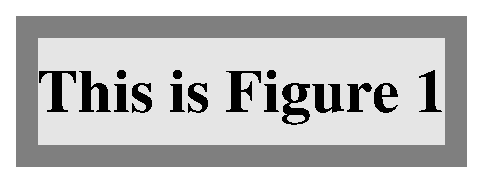
\includegraphics[width=.75\textwidth]{fig1}
  \caption{}
  \label{fig:fig1}
\end{figure}

\begin{figure}
  \centering
  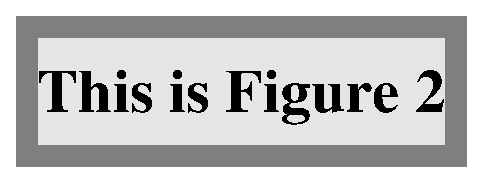
\includegraphics[width=.75\textwidth]{fig2}
  \caption{}
  \label{fig:fig2}
\end{figure}

\begin{figure}
  \centering
  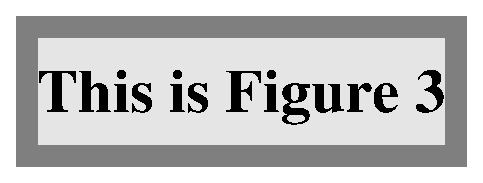
\includegraphics[width=.75\textwidth]{fig3}
  \caption{}
  \label{fig:fig3}
\end{figure}

\bibliographystyle{plain}
\bibliography{/Users/andrewwork/Documents/grad-school/thesis/library}

\end{document}




